% ============================================================
% rapport_final.tex
% Contrôle d'un Jeu par Gestes de la Main — Rapport de Projet
% Vision par Ordinateur — Initiation
% Mars 2026
% Compilable avec : pdflatex rapport_final.tex
% ============================================================

\documentclass[12pt, a4paper]{article}

% --- Encodage & langue ---
\usepackage[T1]{fontenc}
\usepackage[utf8]{inputenc}
\usepackage[french]{babel}

% --- Typographie ---
\usepackage{lmodern}
\usepackage{microtype}

% --- Mise en page ---
\usepackage[top=2.5cm, bottom=2.5cm, left=2.8cm, right=2.8cm]{geometry}
\usepackage{parskip}
\setlength{\parindent}{0pt}

% --- Mathématiques ---
\usepackage{amsmath}
\usepackage{amssymb}

% --- Figures & tableaux ---
\usepackage{graphicx}
\usepackage{float}
\usepackage{caption}
\usepackage{booktabs}
\usepackage{array}
\usepackage{xcolor}

% --- Listings (code source) ---
\usepackage{listings}

\definecolor{codegreen}{rgb}{0.0,0.5,0.0}
\definecolor{codegray}{rgb}{0.5,0.5,0.5}
\definecolor{codepurple}{rgb}{0.55,0.0,0.55}
\definecolor{codeblue}{rgb}{0.0,0.0,0.7}
\definecolor{backcolor}{rgb}{0.97,0.97,0.97}
\definecolor{framecolor}{rgb}{0.75,0.75,0.75}

\lstdefinestyle{python}{
  backgroundcolor=\color{backcolor},
  commentstyle=\color{codegreen}\itshape,
  keywordstyle=\color{codeblue}\bfseries,
  stringstyle=\color{codepurple},
  numberstyle=\tiny\color{codegray},
  basicstyle=\ttfamily\small,
  breakatwhitespace=false,
  breaklines=true,
  captionpos=b,
  keepspaces=true,
  numbers=left,
  numbersep=8pt,
  showspaces=false,
  showstringspaces=false,
  showtabs=false,
  tabsize=4,
  frame=single,
  rulecolor=\color{framecolor},
  language=Python,
  morekeywords={True, False, None, as, import, from, def, return, yield,
                with, lambda, assert, pass, raise, class, in, not, and,
                or, is, elif, global, nonlocal, del, except, finally},
  literate=
    {é}{{\'e}}1 {è}{{\`e}}1 {ê}{{\^e}}1 {ë}{{\"e}}1
    {à}{{\`a}}1 {â}{{\^a}}1 {î}{{\^i}}1 {ô}{{\^o}}1
    {û}{{\^u}}1 {ù}{{\`u}}1 {ç}{{\c{c}}}1 {œ}{{\oe}}1
}

\lstset{style=python}

% --- Liens hypertextes ---
\usepackage{hyperref}
\hypersetup{
  colorlinks=true,
  linkcolor=black,
  citecolor=black,
  urlcolor=blue,
  pdftitle={Contrôle d'un Jeu par Gestes de la Main},
  pdfauthor={Rapport de Projet — Vision par Ordinateur},
}

% --- TikZ (diagrammes) ---
\usepackage{tikz}
\usetikzlibrary{shapes.geometric, arrows.meta, positioning, fit, backgrounds}

% ============================================================
% COMMANDES UTILITAIRES
% ============================================================
\newcommand{\code}[1]{\texttt{\small #1}}
\newcommand{\cls}[1]{\textbf{\texttt{#1}}}

% ============================================================
\begin{document}
% ============================================================

% ============================================================
% PAGE DE TITRE
% ============================================================
\begin{titlepage}
  \centering
  \vspace*{1.5cm}

  {\LARGE\bfseries Contrôle d'un Jeu par Gestes de la Main}\\[0.6em]
  {\Large\bfseries Rapport de Projet}\\[1.5em]

  \rule{\linewidth}{1.5pt}\\[0.5em]
  {\large Vision par Ordinateur --- Initiation}\\[0.3em]
  \rule{\linewidth}{1.5pt}

  \vspace{2cm}

  \begin{tikzpicture}
    \tikzstyle{box} = [rectangle, rounded corners, minimum width=2.8cm,
                       minimum height=0.9cm, text centered,
                       draw=black!60, fill=blue!8, font=\small\ttfamily]
    \tikzstyle{arr} = [->, >=Stealth, thick, color=black!70]

    \node (webcam) [box] {Webcam};
    \node (python) [box, right=1.2cm of webcam] {Python\\(MediaPipe + règles)};
    \node (ws)     [box, right=1.2cm of python] {WebSocket\\(Node.js)};
    \node (game)   [box, right=1.2cm of ws]     {Navigateur\\(Space Invaders)};

    \draw[arr] (webcam) -- (python);
    \draw[arr] (python) -- (ws);
    \draw[arr] (ws)     -- (game);
  \end{tikzpicture}

  \vspace{2cm}

  {\Large Mars 2026}

  \vspace{3cm}

  % --- Abstract ---
  \begin{abstract}
    Ce rapport présente le développement d'un système de contrôle du jeu
    \emph{Space Invaders} par reconnaissance de gestes de la main en temps réel.
    L'architecture finale repose sur un pipeline webcam-Python-WebSocket-navigateur :
    MediaPipe Hands détecte 21 points anatomiques de la main, et le geste est
    reconnu parmi cinq classes (LEFT, RIGHT, FIRE, ENTER, NEUTRAL) puis transmis
    au jeu JavaScript via un serveur WebSocket Node.js.
    Deux approches de classification ont été étudiées : un réseau convolutif (CNN)
    entraîné sur des images brutes 64\(\times\)64, qui n'a atteint que 34,3\,\% de
    précision en raison du problème de fond de scène, et un réseau dense entraîné
    sur des landmarks normalisés, qui atteint 99,6\,\% de précision avec 66 fois
    moins de paramètres et un temps d'entraînement inférieur à la seconde par époque.
    Le système final déployé (\code{cv\_control\_mediapipe.py}) utilise une
    classification par règles géométriques (comptage de doigts et position de la
    paume) plutôt que le réseau dense : cette approche s'avère suffisante pour les
    cinq gestes distincts, plus simple à déployer et plus rapide en production.
    Ce rapport documente l'ensemble de la démarche, les difficultés techniques
    rencontrées, et tire les conclusions pédagogiques sur le choix de la
    représentation en vision par ordinateur.
  \end{abstract}

\end{titlepage}

% ============================================================
% TABLE DES MATIÈRES
% ============================================================
\tableofcontents
\listoffigures
\newpage

% ============================================================
\section{Introduction}
% ============================================================

\subsection{Contexte}

Les interfaces homme-machine classiques --- clavier, souris, manette ---
imposent à l'utilisateur de maîtriser un dispositif physique intermédiaire.
La vision par ordinateur offre la perspective d'interfaces \emph{naturelles}
où le corps devient lui-même le contrôleur. La reconnaissance de gestes de la
main en est l'illustration la plus directe : il suffit de déplacer la main
devant une webcam ordinaire pour envoyer des commandes à un système informatique.

Les applications industrielles et grand public sont nombreuses : contrôle de
présentations, interfaces médicales stériles, jeux vidéo accessibles aux
personnes à mobilité réduite, réalité augmentée, etc. Ce projet s'inscrit dans
ce contexte en appliquant les techniques vues en cours (réseaux convolutifs,
apprentissage supervisé, traitement d'image) à un cas concret et ludique.

\subsection{Objectif du projet}

L'objectif est de contrôler le jeu \emph{Space Invaders} (version JavaScript
exécutée dans un navigateur) en temps réel à partir d'une webcam standard,
sans aucun matériel spécialisé. Cinq gestes doivent être reconnus :

\begin{center}
\begin{tabular}{@{}ll@{}}
  \toprule
  \textbf{Geste} & \textbf{Action dans le jeu} \\
  \midrule
  \cls{LEFT}    & Déplacer le vaisseau à gauche \\
  \cls{RIGHT}   & Déplacer le vaisseau à droite \\
  \cls{FIRE}    & Tirer (poing fermé vers l'avant, knuckles face caméra) \\
  \cls{ENTER}   & Démarrer / valider (paume ouverte, 5 doigts écartés) \\
  \cls{NEUTRAL} & Aucune action (classe de repos) \\
  \bottomrule
\end{tabular}
\end{center}

La contrainte principale est le fonctionnement \emph{en temps réel} sur CPU
standard (sans GPU dédié), ce qui impose des exigences fortes sur la légèreté
du système de détection.

\subsection{Description du jeu et guide des gestes}

\subsubsection{Space Invaders}

Space Invaders est un jeu de tir classique dans lequel le joueur contrôle un
vaisseau spatial se déplaçant horizontalement en bas de l'écran. Des vagues
d'envahisseurs aliens descendent progressivement du haut de l'écran. Le joueur
doit les éliminer en tirant des missiles avant qu'ils n'atteignent le sol ou
ne détruisent le vaisseau. Dans ce projet, les touches du clavier sont
entièrement remplacées par des gestes de la main capturés par la webcam.

\subsubsection{Gestes utilisés}

La figure~\ref{fig:gestes} présente les cinq gestes définis pour contrôler le
jeu. Les squelettes sont reconstruits \emph{directement depuis le vecteur médian}
de chaque classe dans le fichier CSV d'entraînement --- ils reflètent donc
exactement les positions de main réellement apprises par le modèle.

\begin{figure}[H]
  \centering
  \IfFileExists{modeles/images_rapport/grille_gestes.png}{%
    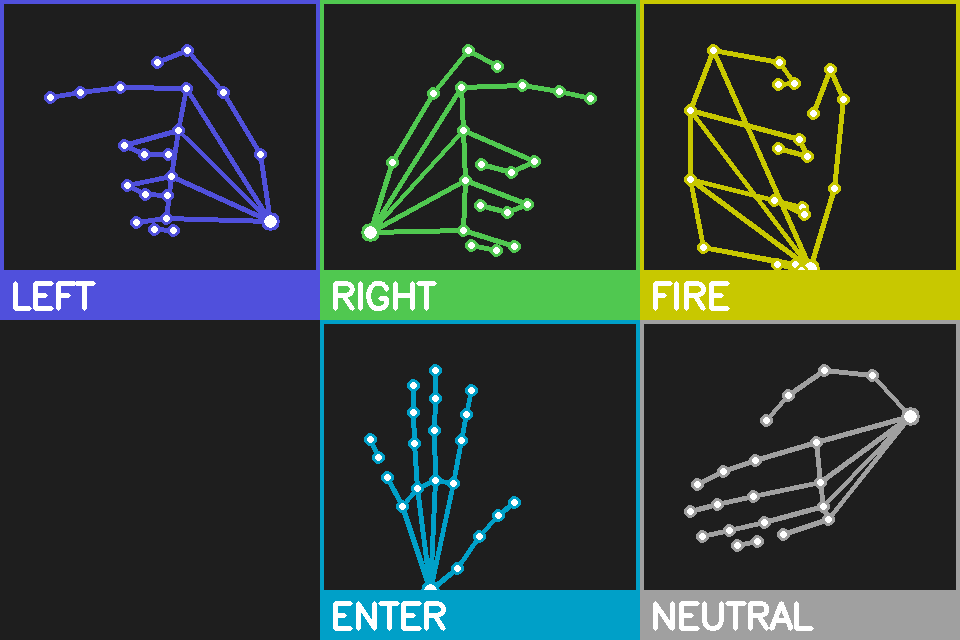
\includegraphics[width=0.90\textwidth]{modeles/images_rapport/grille_gestes.png}
  }{%
    \textit{[Lancer capture\_images\_rapport.py pour générer cette figure]}
  }
  \caption{Cinq gestes de jeu reconstruits depuis les landmarks MediaPipe
           enregistrés à l'entraînement. Chaque squelette représente les
           21 points détectés sur la main réelle du joueur.}
  \label{fig:gestes}
\end{figure}

\begin{center}
\begin{tabular}{@{} c l l l @{}}
  \toprule
  \textbf{Commande} & \textbf{Geste} & \textbf{Description} & \textbf{Effet} \\
  \midrule
  \textsc{left}    & Main à gauche  & 1--3 doigts (index pointé), zone gauche  & Déplacer à gauche \\
  \textsc{right}   & Main à droite  & 1--3 doigts (index pointé), zone droite  & Déplacer à droite \\
  \textsc{fire}    & Poing fermé    & 0 doigt (strict, knuckles face caméra)   & Tirer un missile  \\
  \textsc{enter}   & Paume ouverte  & 4--5 doigts écartés                      & Démarrer / valider \\
  \textsc{neutral} & Position libre & Main posée ou hors cadre  & Aucune action \\
  \bottomrule
\end{tabular}
\end{center}

\subsection{Plan du rapport}

La section~\ref{sec:cnn} présente la première approche tentée --- un CNN sur
images brutes --- et analyse les raisons de son échec. La section~\ref{sec:mediapipe}
explique les algorithmes de MediaPipe Hands qui ont rendu possible la seconde
approche. La section~\ref{sec:landmarks} présente l'approche finale à base de
landmarks, ses résultats et les extraits de code clés. La section~\ref{sec:comparaison}
compare les deux approches de façon synthétique. La section~\ref{sec:architecture}
décrit l'architecture complète du système. La section~\ref{sec:difficultes}
recense les difficultés techniques rencontrées. La section~\ref{sec:conclusion}
conclut et ouvre des perspectives.

% ============================================================
\section{Approche 1 --- CNN sur Images Brutes}
\label{sec:cnn}
% ============================================================

\subsection{Collecte de données}

La première idée naturelle pour de la classification d'images est d'entraîner
un CNN directement sur des photographies de la main. Un script de collecte
(fichier \code{1\_collecter\_images.py}) ouvre la webcam et permet à
l'utilisateur de photographier sa main dans différentes positions, selon deux
modes :

\begin{itemize}
  \item \textbf{Mode automatique} : une image est capturée toutes les 0,4 secondes
        tant que l'utilisateur maintient la position.
  \item \textbf{Mode manuel} : l'utilisateur appuie sur une touche pour déclencher
        la capture.
\end{itemize}

Chaque image est redimensionnée à \(64 \times 64\) pixels en couleur RGB avant
sauvegarde. Le dataset final comprend :

\begin{center}
\begin{tabular}{@{}lrc@{}}
  \toprule
  \textbf{Classe} & \textbf{Images} & \textbf{Représentation} \\
  \midrule
  \cls{LEFT}    & 502 & \rule{4.5cm}{6pt} \\
  \cls{RIGHT}   & 516 & \rule{4.6cm}{6pt} \\
  \cls{FIRE}    & 520 & \rule{4.7cm}{6pt} \\
  \cls{ENTER}   & 520 & \rule{4.7cm}{6pt} \\
  \cls{NEUTRAL} & 463 & \rule{4.2cm}{6pt} \\
  \midrule
  \textbf{Total} & \textbf{2521} & \\
  \bottomrule
\end{tabular}
\end{center}

Les classes sont raisonnablement équilibrées (entre 463 et 520 images),
ce qui évite les biais d'apprentissage liés au déséquilibre.

\subsection{Architecture CNN}

Le réseau convolutif est construit avec Keras (TensorFlow 2.x). Il comprend
trois blocs convolutifs suivi d'une tête de classification dense :

\begin{center}
\begin{tabular}{@{}llcc@{}}
  \toprule
  \textbf{Bloc} & \textbf{Couche} & \textbf{Filtres / Unités} & \textbf{Sortie} \\
  \midrule
  \multirow{5}{*}{Bloc 1}
    & Conv2D (3\(\times\)3, ReLU, same) & 32 & 64\(\times\)64\(\times\)32 \\
    & BatchNormalization & --- & 64\(\times\)64\(\times\)32 \\
    & Conv2D (3\(\times\)3, ReLU, same) & 32 & 64\(\times\)64\(\times\)32 \\
    & MaxPooling2D (2\(\times\)2)        & --- & 32\(\times\)32\(\times\)32 \\
    & Dropout (0.25)                    & --- & 32\(\times\)32\(\times\)32 \\
  \midrule
  \multirow{5}{*}{Bloc 2}
    & Conv2D (3\(\times\)3, ReLU, same) & 64 & 32\(\times\)32\(\times\)64 \\
    & BatchNormalization & --- & 32\(\times\)32\(\times\)64 \\
    & Conv2D (3\(\times\)3, ReLU, same) & 64 & 32\(\times\)32\(\times\)64 \\
    & MaxPooling2D (2\(\times\)2)        & --- & 16\(\times\)16\(\times\)64 \\
    & Dropout (0.25)                    & --- & 16\(\times\)16\(\times\)64 \\
  \midrule
  \multirow{4}{*}{Bloc 3}
    & Conv2D (3\(\times\)3, ReLU, same) & 128 & 16\(\times\)16\(\times\)128 \\
    & BatchNormalization & --- & 16\(\times\)16\(\times\)128 \\
    & MaxPooling2D (2\(\times\)2)        & --- & 8\(\times\)8\(\times\)128 \\
    & Dropout (0.25)                    & --- & 8\(\times\)8\(\times\)128 \\
  \midrule
  \multirow{5}{*}{Dense}
    & Flatten & --- & 8192 \\
    & Dense (ReLU) & 256 & 256 \\
    & BatchNormalization & --- & 256 \\
    & Dropout (0.5) & --- & 256 \\
    & Dense (Softmax) & 5 & 5 \\
  \bottomrule
\end{tabular}
\end{center}

\textbf{Total des paramètres entraînables : 2\,240\,037.}

L'entraînement utilise l'optimiseur Adam (\(\eta = 0{,}001\)) avec deux callbacks :
\code{ReduceLROnPlateau} (facteur 0,5, patience 4) et
\code{EarlyStopping} (patience 8, restauration des meilleurs poids).
Une augmentation de données est appliquée à la volée :
retournements horizontaux, rotations (\(\pm 15\%\)),
zooms (\(\pm 15\%\)), variations de luminosité et de contraste (\(\pm 20\%\)).

L'extrait de code ci-dessous montre la construction du CNN :

\begin{lstlisting}[caption={Architecture CNN (extrait de \texttt{2\_entrainer\_cnn.py})},
                   label=lst:cnn_arch]
modele = models.Sequential([
    # Bloc 1
    layers.Conv2D(32, (3, 3), activation='relu', padding='same',
                  input_shape=(64, 64, 3)),
    layers.BatchNormalization(),
    layers.Conv2D(32, (3, 3), activation='relu', padding='same'),
    layers.MaxPooling2D(2, 2),
    layers.Dropout(0.25),

    # Bloc 2
    layers.Conv2D(64, (3, 3), activation='relu', padding='same'),
    layers.BatchNormalization(),
    layers.Conv2D(64, (3, 3), activation='relu', padding='same'),
    layers.MaxPooling2D(2, 2),
    layers.Dropout(0.25),

    # Bloc 3
    layers.Conv2D(128, (3, 3), activation='relu', padding='same'),
    layers.BatchNormalization(),
    layers.MaxPooling2D(2, 2),
    layers.Dropout(0.25),

    # Tete de classification
    layers.Flatten(),
    layers.Dense(256, activation='relu'),
    layers.BatchNormalization(),
    layers.Dropout(0.5),
    layers.Dense(5, activation='softmax'),
])
\end{lstlisting}

\subsection{Résultats}

L'entraînement s'est déroulé sur 22 époques avant déclenchement de
l'arrêt anticipé. Les performances observées sont :

\begin{itemize}
  \item Meilleure \code{val\_accuracy} : \textbf{34,3\,\%} à l'époque 14.
  \item Niveau du hasard (5 classes équiprobables) : \(1/5 = 20\,\%\).
  \item Comportement général : la courbe d'accuracy reste plate à \(\approx 20\,\%\)
        pendant la quasi-totalité de l'entraînement.
  \item Un pic isolé à 34\,\% aux époques 13--14, suivi d'une rechute immédiate
        vers 20\,\%.
\end{itemize}

\IfFileExists{modeles/courbes_entrainement.png}{%
  \begin{figure}[H]
    \centering
    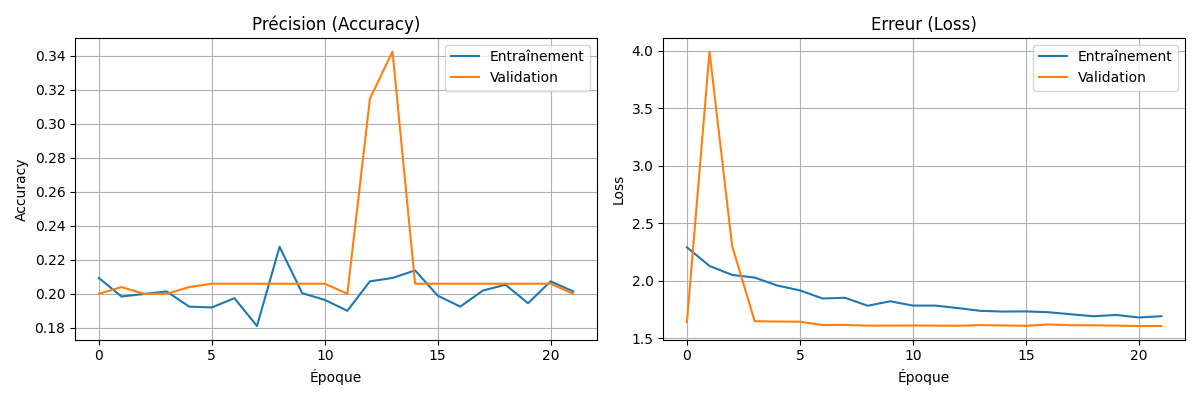
\includegraphics[width=0.92\textwidth]{modeles/courbes_entrainement.png}
    \caption{Courbes d'entraînement du CNN sur images brutes (accuracy et loss).
             La courbe de validation stagne au niveau du hasard (20\,\%).}
    \label{fig:courbes_cnn}
  \end{figure}
}{%
  \begin{figure}[H]
    \centering
    \fbox{\parbox{0.85\textwidth}{\centering\vspace{0.8cm}
      \textit{[Figure non disponible : \texttt{modeles/courbes\_entrainement.png}]}\\
      Courbes d'entraînement du CNN --- val\_accuracy maximale : 34,3\,\%
      \vspace{0.8cm}}}
    \caption{Courbes d'entraînement du CNN (fichier image absent).}
    \label{fig:courbes_cnn}
  \end{figure}
}

\subsection{Analyse de l'échec et implications techniques}
\label{sec:cnn_echec}

\subsubsection{Le problème du fond de scène}

Dans une image \(64 \times 64\) pixels capturée par webcam dans un environnement
non contrôlé, la main n'occupe qu'environ 20\,\% de la surface. Les 80\,\% restants
représentent le fond --- mur, bureau, objets ambiants --- qui varie d'une image
à l'autre et n'est pas corrélé au geste effectué.

En l'absence de segmentation préalable de la main, le CNN est confronté à un
problème de co-occurrence spurieuse : il doit apprendre à ignorer 80\,\% du
signal d'entrée pour se concentrer sur les 20\,\% informatifs. Avec seulement
\(\sim\)500 images par classe, ce n'est pas possible. Le modèle finit par
prédire systématiquement la même classe, ce qui explique la précision de
\(\approx 20\,\%\) --- le niveau attendu pour une prédiction constante sur
5 classes.

\subsubsection{Conditions pour faire fonctionner l'approche images brutes}

Pour que l'approche CNN sur images brutes soit viable, il faudrait réunir au
moins l'une des conditions suivantes :

\begin{enumerate}
  \item \textbf{Volume de données massif} : au minimum 50\,000 images par classe,
        capturées dans des environnements variés (fonds, éclairages, couleurs de
        peau différents).
  \item \textbf{Augmentation de données intensive} : rotations larges, jitter de
        couleur, changements d'éclairage simulés --- bien au-delà de ce qui est
        appliqué ici.
  \item \textbf{Segmentation préalable} : détection et découpe de la main avant
        classification (fond vert / chroma key, ou segmentation sémantique), ce
        qui revient à résoudre un problème de détection avant de résoudre la
        classification.
  \item \textbf{Transfer learning} : partir d'un modèle pré-entraîné sur ImageNet
        (par exemple MobileNetV2) qui possède déjà des représentations génériques
        de formes, et n'affiner que les dernières couches.
\end{enumerate}

\subsubsection{Pourquoi ne pas avoir insisté}

Le rapport coût/bénéfice est défavorable dans le cadre d'un projet académique
à contraintes de temps. La collecte de 50\,000 images par classe demanderait
plusieurs semaines. L'approche par landmarks (section~\ref{sec:landmarks})
résout le problème à la racine en supprimant complètement le fond, est plus
pédagogique --- elle illustre l'importance du choix de la représentation ---
et est plus proche des systèmes industriels réels (MediaPipe, OpenPose, etc.
reposent tous sur des landmarks).

% ============================================================
\section{Algorithmes derrière MediaPipe Hands}
\label{sec:mediapipe}
% ============================================================

\subsection{Vue d'ensemble de MediaPipe}

MediaPipe est un framework open-source développé par Google, conçu pour le
traitement de flux multimédia en temps réel (vidéo, audio, données de capteurs).
Son architecture repose sur des \emph{graphs de calcul} (\code{CalculatorGraph}) :
un pipeline déclaratif où chaque nœud (\emph{Calculator}) effectue une opération
atomique (redimensionnement, inférence de réseau, filtrage temporel), et les
données transitent sous forme de paquets horodatés entre les nœuds.

Pour la détection de mains, MediaPipe Hands enchaîne deux modèles d'inférence :
BlazePalm (détection) et Hand Landmark Model (estimation de poses).

\subsection{BlazePalm --- Détection de la main}

BlazePalm est un détecteur de mains léger basé sur l'architecture
\emph{Single-Shot Detector} (SSD). Son fonctionnement se déroule en deux étapes :

\begin{enumerate}
  \item \textbf{Détection par ancres} (\emph{anchor-based detection}) : un ensemble
        d'ancres prédéfinies, adaptées aux proportions allongées des mains (contrairement
        aux ancres rectangulaires standard), couvrent l'espace des positions et
        tailles possibles. Pour chaque ancre, le réseau prédit une probabilité
        de présence de main et un décalage de position.
  \item \textbf{Prédiction de bounding box} : les ancres à forte probabilité sont
        raffinées par régression pour produire la boîte englobante précise de la paume.
        Une suppression des non-maxima (NMS) élimine les détections redondantes.
\end{enumerate}

Le modèle a été entraîné par Google sur des millions d'images annotées de mains.
Il fonctionne sur CPU mobile à environ 30 FPS. Les paramètres exposés à
l'utilisateur sont :

\begin{itemize}
  \item \code{min\_hand\_detection\_confidence} : seuil de confiance minimum pour
        considérer une détection valide (valeur utilisée dans ce projet : 0,6).
  \item \code{min\_tracking\_confidence} : seuil pour maintenir le suivi d'une main
        déjà détectée d'une frame à l'autre (valeur : 0,5).
\end{itemize}

En mode \code{VIDEO}, une fois la main détectée, BlazePalm n'est pas réexécuté
à chaque frame : un algorithme de suivi (\emph{tracker}) léger maintient la
bounding box entre les frames, ce qui réduit considérablement le coût de calcul.

\subsection{Hand Landmark Model --- 21 points clés}

Une fois la paume localisée par BlazePalm, un second réseau convolutif (de type
MobileNet allégé) prédit les positions de 21 points anatomiques (\emph{landmarks})
dans l'image recadrée sur la paume.

\begin{figure}[H]
  \centering
  \begin{tikzpicture}[scale=0.9]
    % Paume stylisée
    \draw[thick, fill=gray!10] (0,0) ellipse (1.2cm and 1.5cm);
    % Doigts
    \foreach \x/\name in {-0.9/P, -0.45/A, 0/M, 0.45/N, 0.9/O} {
      \draw[thick] (\x, 1.3) -- (\x, 2.8);
    }
    % Points
    \filldraw[blue] (0, -1.3) circle (3pt) node[below, font=\tiny] {0 Poignet};
    \foreach \x/\y/\n in {-0.9/1.4/5, -0.45/1.4/9, 0/1.4/13, 0.45/1.4/17, 0.9/1.4/1} {
      \filldraw[red] (\x, \y) circle (2.5pt) node[right, font=\tiny] {\n};
    }
    \foreach \x/\y/\n in {-0.9/1.9/6, -0.45/1.9/10, 0/1.9/14, 0.45/1.9/18, 0.9/1.9/2} {
      \filldraw[orange] (\x, \y) circle (2.5pt) node[right, font=\tiny] {\n};
    }
    \foreach \x/\y/\n in {-0.9/2.3/7, -0.45/2.3/11, 0/2.3/15, 0.45/2.3/19, 0.9/2.3/3} {
      \filldraw[green!60!black] (\x, \y) circle (2.5pt) node[right, font=\tiny] {\n};
    }
    \foreach \x/\y/\n in {-0.9/2.75/8, -0.45/2.75/12, 0/2.75/16, 0.45/2.75/20, 0.9/2.75/4} {
      \filldraw[purple] (\x, \y) circle (2.5pt) node[right, font=\tiny] {\n};
    }
  \end{tikzpicture}
  \caption{Schéma des 21 landmarks MediaPipe Hands (simplifié). Point 0 = poignet,
           1--4 = pouce, 5--8 = index, 9--12 = majeur, 13--16 = annulaire, 17--20 = auriculaire.}
  \label{fig:landmarks_schema}
\end{figure}

Les 21 points sont organisés comme suit :

\begin{center}
\begin{tabular}{@{}cll@{}}
  \toprule
  \textbf{Indice(s)} & \textbf{Anatomie} & \textbf{Articulation} \\
  \midrule
  0  & Poignet & --- \\
  1, 5, 9, 13, 17 & Base des doigts & MCP \\
  2, 6, 10, 14, 18 & Première articulation & PIP \\
  3, 7, 11, 15, 19 & Deuxième articulation & DIP \\
  4, 8, 12, 16, 20 & Bouts des doigts & Tip \\
  \bottomrule
\end{tabular}
\end{center}

Chaque landmark est fourni avec trois coordonnées :
\begin{itemize}
  \item \(x, y \in [0, 1]\) : position normalisée dans l'image (fraction de la largeur
        et de la hauteur).
  \item \(z\) : profondeur relative estimée par rapport au poignet --- un \(z\) positif
        indique un point plus proche de la caméra que le poignet, un \(z\) négatif
        indique un point plus éloigné.
\end{itemize}

En conditions normales, la précision du modèle est sub-pixel, ce qui en fait une
représentation très riche pour la classification de gestes.

\subsection{Aspects d'implémentation côté code}

La version de MediaPipe utilisée dans ce projet (\(\geq 0.10\)) impose d'utiliser
la \emph{Tasks API}, une API modernisée qui remplace l'ancienne interface
\code{mp.solutions.hands} (désormais supprimée dans les versions récentes).

\begin{lstlisting}[caption={Initialisation de MediaPipe HandLandmarker (Tasks API)},
                   label=lst:mediapipe_init]
import mediapipe as mp
from mediapipe.tasks import python as mp_python
from mediapipe.tasks.python import vision as mp_vision

base_options = mp_python.BaseOptions(model_asset_path=MODEL_PATH)
options = mp_vision.HandLandmarkerOptions(
    base_options=base_options,
    running_mode=mp_vision.RunningMode.VIDEO,
    num_hands=1,
    min_hand_detection_confidence=0.6,
    min_hand_presence_confidence=0.5,
    min_tracking_confidence=0.5,
)
landmarker = mp_vision.HandLandmarker.create_from_options(options)
\end{lstlisting}

Le mode \code{VIDEO} est crucial : il active le suivi temporel entre frames,
ce qui améliore la stabilité et la fluidité de la détection. La méthode
\code{detect\_for\_video(mp\_image, timestamp\_ms)} requiert un timestamp
strictement croissant à chaque appel, ce que l'on assure en mesurant le temps
écoulé depuis le démarrage :

\begin{lstlisting}[caption={Boucle de capture et détection MediaPipe},
                   label=lst:mediapipe_loop]
start_ms = int(time.time() * 1000)
while True:
    ret, frame = cap.read()
    frame  = cv2.flip(frame, 1)          # miroir horizontal
    ts_ms  = int(time.time() * 1000) - start_ms  # timestamp croissant

    rgb    = cv2.cvtColor(frame, cv2.COLOR_BGR2RGB)
    mp_img = mp.Image(image_format=mp.ImageFormat.SRGB, data=rgb)
    result = landmarker.detect_for_video(mp_img, ts_ms)

    if result.hand_landmarks:
        lm = result.hand_landmarks[0]  # liste de 21 NormalizedLandmark
\end{lstlisting}

Le modèle utilisé est le modèle \code{float16}, un compromis entre la précision
du modèle \code{float32} et la vitesse du modèle \code{lite}, adapté à une
exécution CPU en temps réel.

% ============================================================
\section{Approche 2 --- Réseau Dense sur Landmarks}
\label{sec:landmarks}
% ============================================================

\subsection{Principe et motivation}

Plutôt que de donner les pixels bruts au classifieur, l'approche landmarks
exploite la détection de MediaPipe pour réduire la représentation de la main
à ses 21 points anatomiques. Cette réduction est fondamentale :

\[
64 \times 64 \times 3 = 12\,288 \text{ valeurs} \quad \longrightarrow \quad
21 \times 3 = 63 \text{ coordonnées}
\]

Cette représentation compacte est \textbf{invariante par construction} au fond
de la scène, à l'éclairage, à la couleur de peau et à la distance à la caméra
(après normalisation). Le classifieur n'a plus à résoudre le problème difficile
de la détection de la main dans l'image --- ce travail est délégué à MediaPipe.
Il doit uniquement discriminer des configurations géométriques en 63 dimensions.

\subsection{Normalisation des landmarks}

La normalisation est une étape cruciale pour rendre les coordonnées invariantes
à la position et à la taille de la main dans l'image. Elle se déroule en deux
opérations successives :

\begin{enumerate}
  \item \textbf{Centrage} : soustraction de la position du poignet (point 0),
        ce qui ramène la configuration dans un repère centré sur le poignet,
        indépendant de la position absolue de la main dans l'image.
  \item \textbf{Normalisation d'échelle} : division par la distance maximale
        entre le poignet et tout autre point, ce qui rend la représentation
        indépendante de la taille de la main (distance à la caméra).
\end{enumerate}

Formellement, en notant \(\mathbf{p}_i = (x_i, y_i, z_i)\) les coordonnées brutes
du point \(i\) :

\begin{equation}
  \mathbf{p}'_i = \frac{\mathbf{p}_i - \mathbf{p}_0}
                       {\displaystyle\max_{j \in \{0,\ldots,20\}} \|\mathbf{p}_j - \mathbf{p}_0\|_\infty}
  \label{eq:normalisation}
\end{equation}

Le résultat est un vecteur de 63 valeurs dans \([-1, +1]\) représentant la
\emph{forme pure} de la main, indépendamment de son contexte spatial.

\begin{lstlisting}[caption={Fonction de normalisation des landmarks (extrait de
                   \texttt{3\_collecter\_landmarks.py} et \texttt{5\_jouer\_avec\_cnn.py})},
                   label=lst:normalisation]
def normaliser_landmarks(landmarks):
    """
    Normalise les 21 landmarks par rapport au poignet (point 0).
    Retourne un vecteur de 63 valeurs dans [-1, +1].
    """
    # Extraire les coordonnees x, y, z
    pts = np.array([[lm.x, lm.y, lm.z] for lm in landmarks],
                   dtype=np.float32)

    # Centrer sur le poignet (point 0)
    pts -= pts[0]

    # Normaliser par la distance maximale (norme infinie)
    scale = np.max(np.abs(pts))
    if scale > 0:
        pts /= scale

    return pts.flatten()   # vecteur de 63 valeurs
\end{lstlisting}

\subsection{Architecture du réseau dense}

Le classifieur est un réseau entièrement connecté (\emph{fully connected network}
ou MLP) à trois couches cachées. Sa petite taille est rendue possible par la
richesse de la représentation en entrée : les 63 coordonnées normalisées
encodent déjà efficacement la configuration de la main.

\begin{center}
\begin{tabular}{@{}llcc@{}}
  \toprule
  \textbf{Numéro} & \textbf{Couche} & \textbf{Activation} & \textbf{Sorties} \\
  \midrule
  1 & Input & --- & 63 \\
  2 & Dense & ReLU & 128 \\
  3 & BatchNormalization & --- & 128 \\
  4 & Dropout (0,3) & --- & 128 \\
  5 & Dense & ReLU & 128 \\
  6 & BatchNormalization & --- & 128 \\
  7 & Dropout (0,3) & --- & 128 \\
  8 & Dense & ReLU & 64 \\
  9 & BatchNormalization & --- & 64 \\
  10 & Dropout (0,2) & --- & 64 \\
  11 & Dense & Softmax & 5 \\
  \bottomrule
\end{tabular}
\end{center}

\textbf{Total des paramètres : 33\,925} --- soit 66 fois moins que le CNN.

\begin{lstlisting}[caption={Architecture du réseau dense (extrait de
                   \texttt{4\_entrainer\_landmarks.py})},
                   label=lst:mlp_arch]
model = keras.Sequential([
    keras.Input(shape=(63,)),

    keras.layers.Dense(128, activation='relu'),
    keras.layers.BatchNormalization(),
    keras.layers.Dropout(0.3),

    keras.layers.Dense(128, activation='relu'),
    keras.layers.BatchNormalization(),
    keras.layers.Dropout(0.3),

    keras.layers.Dense(64, activation='relu'),
    keras.layers.BatchNormalization(),
    keras.layers.Dropout(0.2),

    keras.layers.Dense(5, activation='softmax'),
])

model.compile(
    optimizer=keras.optimizers.Adam(learning_rate=0.001),
    loss='sparse_categorical_crossentropy',
    metrics=['accuracy'],
)
\end{lstlisting}

\subsection{Collecte de données et entraînement}

Le script \code{3\_collecter\_landmarks.py} remplace la collecte d'images par
une collecte de vecteurs de landmarks. Pour chaque frame avec une main détectée,
on extrait et normalise les 63 coordonnées, puis on les sauvegarde dans un fichier
CSV avec la classe correspondante. La collecte est plus rapide : le CSV final
est quelques centaines de Ko, contre plusieurs centaines de Mo pour les images.

\textbf{Dataset final :}

\begin{center}
\begin{tabular}{@{}lrr@{}}
  \toprule
  \textbf{Classe} & \textbf{Landmarks (train+val)} & \textbf{Validation (20\,\%)} \\
  \midrule
  \cls{ENTER}   & 500 & 100 \\
  \cls{FIRE}    & 501 & 101 \\
  \cls{LEFT}    & 500 & 100 \\
  \cls{NEUTRAL} & 503 & 101 \\
  \cls{RIGHT}   & 500 & 100 \\
  \midrule
  \textbf{Total} & \textbf{2504} & \textbf{501} \\
  \bottomrule
\end{tabular}
\end{center}

Le split 80/20 avec stratification donne 2003 échantillons d'entraînement et
501 de validation.

\subsection{Résultats}

L'entraînement s'est terminé à l'époque 28 (sur 50 maximum), avec arrêt
anticipé. Les résultats sont remarquables :

\begin{itemize}
  \item \textbf{Meilleure \code{val\_accuracy} : 99,6\,\%} à l'époque 13.
  \item Temps par époque : \textbf{moins d'une seconde} (CPU, sans GPU).
  \item Seulement \textbf{2 erreurs} sur 501 échantillons de validation.
\end{itemize}

\IfFileExists{modeles/courbes_landmarks.png}{%
  \begin{figure}[H]
    \centering
    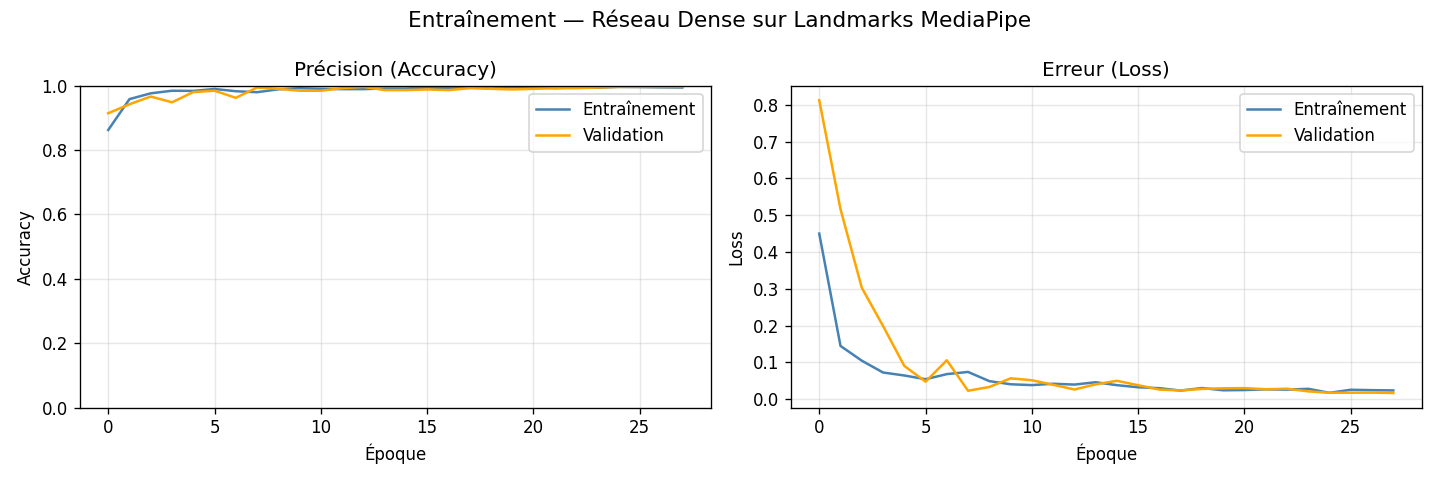
\includegraphics[width=0.92\textwidth]{modeles/courbes_landmarks.png}
    \caption{Courbes d'entraînement du réseau dense sur landmarks.
             La validation converge vers 99,6\,\% en moins de 15 époques.}
    \label{fig:courbes_landmarks}
  \end{figure}
}{%
  \begin{figure}[H]
    \centering
    \fbox{\parbox{0.85\textwidth}{\centering\vspace{0.8cm}
      \textit{[Figure non disponible : \texttt{modeles/courbes\_landmarks.png}]}\\
      Courbes d'entraînement du réseau dense --- val\_accuracy maximale : 99,6\,\%
      \vspace{0.8cm}}}
    \caption{Courbes d'entraînement du réseau dense (fichier image absent).}
    \label{fig:courbes_landmarks}
  \end{figure}
}

\textbf{Matrice de confusion} (sur les 501 échantillons de validation) :

\begin{center}
\begin{tabular}{@{}l|ccccc|c@{}}
  \toprule
   & \textbf{ENTER} & \textbf{FIRE} & \textbf{LEFT} & \textbf{NEUTRAL} & \textbf{RIGHT} & \textbf{Total} \\
  \midrule
  \textbf{ENTER}   & \textbf{100} & 0 & 0 & 0 & 0 & 100 \\
  \textbf{FIRE}    & 0 & \textbf{100} & 0 & 0 & 0 & 100 \\
  \textbf{LEFT}    & 0 & 0 & \textbf{100} & 0 & 0 & 100 \\
  \textbf{NEUTRAL} & 0 & 1 & 1 & \textbf{99} & 0 & 101 \\
  \textbf{RIGHT}   & 0 & 0 & 0 & 0 & \textbf{100} & 100 \\
  \bottomrule
\end{tabular}
\end{center}

Les deux seules erreurs concernent la classe NEUTRAL : un échantillon est
confondu avec FIRE et un avec LEFT. Ces confusions sont cohérentes : une
main en position neutre peut ressembler à une paume partiellement ouverte%
\footnote{Note : dans les données d'entraînement utilisées ici, la classe FIRE
correspondait à la paume ouverte~; cette définition a été révisée après les
tests utilisateur, FIRE désignant désormais le poing fermé (knuckles face
caméra) dans le système final déployé.}
(FIRE) ou à une main en position latérale (LEFT) selon l'angle de prise de vue.

\subsection{Mécanisme de stabilisation temporelle}

Pour éviter les faux positifs liés à des fluctuations instantanées de la
prédiction, un mécanisme de \emph{buffer de stabilisation} exige que le même
geste soit prédit deux frames consécutives avant d'être envoyé. Un seuil de
confiance de 0,75 filtre également les prédictions incertaines.

\begin{lstlisting}[caption={Stabilisation temporelle des prédictions (extrait de
                   \texttt{5\_jouer\_avec\_cnn.py})},
                   label=lst:stabilisation]
SEUIL_CONFIANCE = 0.75
STABILITE       = 2        # nombre de frames consecutives requis

buffer = []

# Dans la boucle principale :
probs_all = model.predict(vecteur, verbose=0)[0]
idx       = int(np.argmax(probs_all))
confiance = float(probs_all[idx])
geste     = CLASSES[idx] if confiance >= SEUIL_CONFIANCE else None

# Stabilisation
buffer.append(geste)
if len(buffer) > STABILITE:
    buffer.pop(0)

geste_stable = (
    buffer[-1]
    if len(buffer) == STABILITE and len(set(buffer)) == 1
    else None
)
\end{lstlisting}

% ============================================================
\section{Comparaison des Deux Approches}
\label{sec:comparaison}
% ============================================================

\begin{center}
\begin{tabular}{@{}lcc@{}}
  \toprule
  \textbf{Critère} & \textbf{CNN Images brutes} & \textbf{Dense Landmarks} \\
  \midrule
  Précision (validation) & 34,3\,\% & \textbf{99,6\,\%} \\
  Paramètres & 2\,240\,037 & \textbf{33\,925} \\
  Données nécessaires & 50\,000+ & \textbf{\(\sim\)500} \\
  Temps par époque & \(\sim\)16\,s & \textbf{$<$ 1\,s} \\
  Sensibilité au fond & Critique & \textbf{Nulle} \\
  Sensibilité à l'éclairage & Oui & \textbf{Non} \\
  Sensibilité couleur de peau & Oui & \textbf{Non} \\
  Pré-traitement requis & Segmentation de la main & Normalisation simple \\
  Généralisation à d'autres utilisateurs & Faible & \textbf{Bonne} \\
  Adapté au temps réel sur CPU & Non & \textbf{Oui} \\
  Complexité d'implémentation & Élevée & \textbf{Modérée} \\
  Taille du dataset (Mo) & \(\sim\)300 & \textbf{\(\sim\)0,5} \\
  \bottomrule
\end{tabular}
\end{center}

La supériorité de l'approche landmarks sur images brutes est totale dans ce
contexte. Elle illustre un principe général en apprentissage automatique :
\textbf{le choix de la représentation est souvent plus déterminant que
le choix de l'algorithme}. En fournissant au classifieur une représentation
qui encode directement l'information pertinente (la géométrie de la main),
on résout le problème avec des ordres de grandeur moins de données et de calcul.

% ============================================================
\section{Architecture du Système Complet}
\label{sec:architecture}
% ============================================================

\subsection{Pipeline de traitement en temps réel}

Le système complet comprend trois processus communicants :

\begin{enumerate}
  \item \textbf{Script Python} (\code{cv\_control\_mediapipe.py}) : capture vidéo,
        détection MediaPipe, classification par règles géométriques, envoi WebSocket.
  \item \textbf{Serveur Node.js} (\code{server.js}) : relais WebSocket entre Python
        et le navigateur, gestion des événements clavier.
  \item \textbf{Navigateur} (\code{index.html} + \code{game.bundle.js}) : jeu
        Space Invaders, écoute des événements clavier simulés.
\end{enumerate}

Le script déployé en production est \code{cv\_control\_mediapipe.py}. Il utilise
une \textbf{classification par règles géométriques} (comptage de doigts étendus
et position horizontale de la paume) plutôt qu'un réseau de neurones chargé~:
cette approche est suffisante pour distinguer cinq gestes bien distincts, plus
simple à déployer et plus rapide. Le réseau dense (\code{5\_jouer\_avec\_cnn.py}),
bien que validé expérimentalement à 99,6\,\%, constitue une contribution
scientifique documentée dans ce rapport (section~\ref{sec:landmarks}).

Le pipeline de traitement du script déployé, frame par frame, est le suivant :

\begin{center}
\begin{tikzpicture}[
  node distance=0.6cm and 0.4cm,
  block/.style={rectangle, rounded corners, draw=black!60, fill=blue!7,
                minimum width=3.5cm, minimum height=0.75cm,
                text centered, font=\small},
  arrow/.style={->, >=Stealth, thick}
]
  \node (cam)   [block] {1. Webcam \(\rightarrow\) frame OpenCV};
  \node (flip)  [block, below=of cam] {2. Flip miroir (cv2.flip)};
  \node (conv)  [block, below=of flip] {3. BGR \(\rightarrow\) RGB \(\rightarrow\) mp.Image};
  \node (mp)    [block, below=of conv] {4. MediaPipe detect\_for\_video};
  \node (rules) [block, below=of mp]  {5. Classification par règles (count\_fingers + position)};
  \node (ws)    [block, below=of rules]{6. asyncio + WebSocket};
  \node (node)  [block, below=of ws]  {7. Node.js : hold timer (180\,ms)};
  \node (game)  [block, below=of node]{8. Navigateur : keydown/keyup};

  \foreach \a/\b in {cam/flip, flip/conv, conv/mp, mp/rules, rules/ws, ws/node, node/game}
    \draw[arrow] (\a) -- (\b);
\end{tikzpicture}
\end{center}

\subsection{Architecture Python du script expérimental (\texttt{5\_jouer\_avec\_cnn.py})}

Cette section décrit l'architecture de \code{5\_jouer\_avec\_cnn.py}, le script
expérimental qui charge et exécute le réseau dense. Il n'est \textbf{pas} le
script déployé en production (voir section précédente), mais son architecture
illustre des contraintes techniques importantes.

Un problème fondamental est apparu lors du développement : asyncio, la
bibliothèque Python pour les coroutines asynchrones, et les appels synchrones
de MediaPipe et TensorFlow sont incompatibles. Un appel \code{detect\_for\_video}
ou \code{model.predict} bloque le thread asyncio, empêchant l'envoi des commandes
WebSocket et provoquant des latences inacceptables.

La solution adoptée dans \code{5\_jouer\_avec\_cnn.py} est une \textbf{architecture
à deux threads} :

\begin{itemize}
  \item \textbf{Thread principal} : boucle vidéo synchrone (capture, MediaPipe,
        CNN, dépôt des commandes dans une \code{queue.Queue}).
  \item \textbf{Thread secondaire} (daemon) : connexion WebSocket via la bibliothèque
        synchrone \code{websocket-client}, lecture de la queue, envoi des commandes.
\end{itemize}

En revanche, \code{cv\_control\_mediapipe.py} (le script déployé) utilise
\code{asyncio} combiné à \code{websockets}~: comme il n'effectue aucun appel
\code{model.predict} (pas de réseau chargé), la boucle événementielle asyncio
n'est pas bloquée et cette architecture plus simple suffit.

\begin{lstlisting}[caption={Architecture deux threads pour le WebSocket (extrait de
                   \texttt{5\_jouer\_avec\_cnn.py} --- script expérimental)},
                   label=lst:threading]
import websocket          # websocket-client (synchrone, thread-safe)
import threading
import queue

cmd_queue   = queue.Queue(maxsize=20)
ws_connecte = threading.Event()

def ws_worker():
    """Thread dedie au WebSocket --- jamais bloque par la video."""
    def on_open(ws):
        ws_connecte.set()
        while True:
            try:
                cmd = cmd_queue.get(timeout=0.5)
                if cmd is None:    # signal d'arret
                    ws.close()
                    return
                ws.send(cmd)
            except queue.Empty:
                pass

    ws_app = websocket.WebSocketApp(
        WS_URI, on_open=on_open,
        on_error=lambda ws, e: print(f"WS erreur: {e}"),
        on_close=lambda ws, c, m: ws_connecte.clear(),
    )
    ws_app.run_forever()

# Demarrer le thread WebSocket en arriere-plan
t = threading.Thread(target=ws_worker, daemon=True)
t.start()
ws_connecte.wait(timeout=5)  # attendre la connexion

def envoyer(cmd):
    """Envoie non bloquant dans la queue."""
    try:
        cmd_queue.put_nowait(cmd)
    except queue.Full:
        pass
\end{lstlisting}

\subsection{Mécanisme hold timer du serveur Node.js}

Un problème de timing a été identifié côté serveur : les commandes de mouvement
(LEFT, RIGHT) doivent être maintenues tant que le geste est détecté, mais
le serveur ne peut pas savoir quand le geste se termine.

La solution est un \textbf{hold timer} : à chaque réception d'une commande
de mouvement, le serveur envoie un \code{keydown} (si la touche n'est pas
déjà enfoncée), puis programme un \code{keyup} après 180\,ms. Si la même
commande arrive à nouveau avant l'expiration du timer, le timer est réinitialisé.
La touche est ainsi maintenue enfoncée tant que les commandes arrivent à un
débit supérieur à une toutes les 180\,ms.

\begin{lstlisting}[caption={Mécanisme hold timer dans \texttt{server.js} (Node.js)},
                   label=lst:holdtimer,
                   language=Java]
const HOLD_TIMEOUT = 180;   // ms

if (HOLD_COMMANDS.has(command)) {
    // Envoyer keydown seulement si pas deja enfonce
    if (!heldKeys[command]) {
        broadcast(wss, ws, { type: 'keydown', keyCode });
        heldKeys[command] = true;
    }
    // Reinitialiser le timer de relachement
    clearTimeout(holdTimers[command]);
    holdTimers[command] = setTimeout(() => {
        broadcast(wss, ws, { type: 'keyup', keyCode });
        heldKeys[command] = false;
    }, HOLD_TIMEOUT);
}
\end{lstlisting}

% ============================================================
\section{Difficultés Rencontrées}
\label{sec:difficultes}
% ============================================================

Ce projet a été émaillé de difficultés techniques significatives. Leur résolution
a constitué une part importante de l'apprentissage.

\subsection{Suppression de \texttt{mediapipe.solutions} dans les versions récentes}

L'API historique \code{mp.solutions.hands} a été supprimée dans
MediaPipe \(\geq 0.10.14\). Tous les tutoriels et exemples trouvés en ligne
utilisaient l'ancienne API, ce qui a provoqué des erreurs \code{AttributeError}
immédiatement au lancement. La migration vers la Tasks API
(\code{mediapipe.tasks.python.vision.HandLandmarker}) a nécessité une compréhension
complète de la nouvelle interface, significativement différente de l'ancienne.

\subsection{Port WebSocket déjà occupé (\texttt{EADDRINUSE 8765})}

Lors des redémarrages fréquents pendant le développement, le port 8765 restait
parfois occupé par des processus Node.js zombies (non terminés proprement).
L'erreur \code{EADDRINUSE} bloquait tout redémarrage. La résolution a impliqué
l'identification et la terminaison manuelle des processus zombies, et l'ajout
d'une gestion propre des signaux d'arrêt dans le serveur.

\subsection{CNN bloqué à 20\,\% d'accuracy}

Décrit en détail dans la section~\ref{sec:cnn_echec}, ce problème a été le plus
coûteux en temps. Le diagnostic a pris plusieurs sessions d'entraînement avant
de comprendre que le fond de scène, et non la qualité du modèle ou des
hyperparamètres, était la cause fondamentale.

\subsection{Erreur de labellisation des landmarks}

Lors de la collecte initiale des landmarks, 47 échantillons de la classe RIGHT
ont été capturés par inadvertance avec le geste FIRE (la touche de changement
de classe avait été manquée). Ces erreurs de labellisation ont été détectées
par analyse de la matrice de confusion (confusion anormalement élevée entre
RIGHT et FIRE) et corrigées en filtrant le CSV avec pandas :

\begin{lstlisting}[caption={Détection et correction d'erreurs de labellisation (pandas)},
                   label=lst:correction]
import pandas as pd

df = pd.read_csv("data_landmarks/landmarks.csv")
print(df['classe'].value_counts())

# Supprimer les lignes erronees identifiees
# (par exemple, les 47 premieres lignes RIGHT)
df = df.drop(df[df['classe'] == 'RIGHT'].head(47).index)
df.to_csv("data_landmarks/landmarks_corrige.csv", index=False)
\end{lstlisting}

\subsection{Incompatibilité asyncio / MediaPipe / TensorFlow}

La première version du script de jeu utilisait \code{asyncio} et
\code{websockets} (asynchrone). Les appels synchrones \code{detect\_for\_video}
et \code{model.predict} bloquaient la boucle d'événements asyncio, rendant
le WebSocket non réactif. La latence dépassait plusieurs secondes. La migration
vers une architecture à deux threads (section~\ref{sec:architecture}) a résolu
le problème.

\subsection{Timing keydown/keyup : conflit entre cooldowns}

Le premier serveur envoyait un \code{keydown} suivi d'un \code{keyup} après
100\,ms pour chaque commande. Avec un cooldown Python de 50\,ms entre les
envois de commandes, le serveur envoyait \code{keyup} juste avant que la
commande suivante n'arrive : la touche se relâchait systématiquement avant
le \code{keydown} suivant, rendant le mouvement saccadé. Le hold timer de
180\,ms (section~\ref{sec:architecture}) a résolu ce problème en desynchronisant
le relâchement de la touche de l'arrivée des commandes.

\subsection{Encodage terminal Windows : \texttt{UnicodeEncodeError}}

Les scripts affichaient des barres de progression avec le caractère Unicode
\code{█} (U+2588). Sur Windows avec l'encodage cp1252 du terminal,
\code{UnicodeEncodeError} était levée. La solution a été de remplacer ces
caractères par des équivalents ASCII, ou de forcer l'encodage UTF-8 du
terminal via \code{PYTHONIOENCODING=utf-8}.

\subsection{Latéralité inversée après flip miroir}

MediaPipe détermine la latéralité (main gauche/droite) en analysant l'orientation
anatomique de la main. Après le flip miroir horizontal appliqué pour que la
webcam fonctionne comme un miroir, la latéralité fournie par MediaPipe est
inversée (la main droite de l'utilisateur est détectée comme gauche). Plutôt
que de s'appuyer sur l'attribut \code{handedness}, la détection des gestes
utilise une méthode géométrique robuste basée sur les positions relatives des
doigts (la position \(y\) de l'extrémité du doigt par rapport à l'articulation PIP),
indépendante de la latéralité.

% ============================================================
\section{Conclusion}
\label{sec:conclusion}
% ============================================================

\subsection{Bilan technique}

Ce projet démontre de façon concrète que l'approche landmarks est largement
supérieure à l'approche par images brutes pour la reconnaissance de gestes
en temps réel sur CPU. Le réseau dense sur landmarks atteint 99,6\,\% de
précision avec 66 fois moins de paramètres, 100 fois moins de données et
des temps d'entraînement inférieurs à la seconde par époque.

Le \textbf{système final déployé} (\code{cv\_control\_mediapipe.py}) va plus
loin encore : il n'utilise pas le réseau entraîné, mais une \textbf{classification
par règles géométriques} directement sur les landmarks MediaPipe (comptage de
doigts étendus, position horizontale de la paume). Pour cinq gestes bien distincts,
cette approche s'avère aussi efficace que le réseau dense, tout en étant plus
simple à déployer et plus rapide. Le réseau dense reste une contribution
scientifique valide, documentée dans la section~\ref{sec:landmarks}.

Plus fondamentalement, ce projet illustre que \textbf{le choix de la
représentation est plus important que le choix du modèle}. Un réseau dense
simple --- ou même des règles géométriques --- sur une bonne représentation
surpasse largement un CNN sophistiqué sur des pixels bruts, dans ce contexte.

\subsection{Ce qu'on a appris sur la vision par ordinateur appliquée}

\begin{itemize}
  \item \textbf{La détection et la classification sont deux problèmes distincts}.
        Utiliser un détecteur spécialisé (MediaPipe) pour résoudre la détection
        et ne demander au classifieur que la classification est une division du
        travail efficace.
  \item \textbf{Les landmarks sont une représentation puissante et générale}
        pour les gestes corporels. C'est l'approche adoptée par les systèmes
        industriels (MediaPipe, OpenPose, AlphaPose).
  \item \textbf{L'ingénierie système est aussi importante que le modèle} : le
        hold timer, l'architecture deux threads, la gestion des timestamps --- autant
        de problèmes qui n'apparaissent pas dans les tutoriels mais sont
        incontournables en pratique.
  \item \textbf{Le diagnostic des échecs est une compétence cruciale} : comprendre
        pourquoi le CNN était bloqué à 20\,\% a demandé une analyse approfondie du
        problème de fond, qui n'était pas évidente a priori.
\end{itemize}

\subsection{Limites}

\begin{itemize}
  \item \textbf{Dépendance à l'utilisateur} : le modèle est entraîné sur les
        gestes d'un seul utilisateur. Les variations inter-individuelles (taille
        de la main, habitudes de geste) peuvent dégrader les performances pour
        d'autres utilisateurs sans recollecte de données.
  \item \textbf{Nombre limité de gestes} : cinq gestes simples, sans gestes
        combinés ni mouvements dynamiques (gestes de balayage, vitesse).
  \item \textbf{Condition d'éclairage extrêmes} : en très faible éclairage,
        MediaPipe peut perdre la détection de la main.
  \item \textbf{Single-hand} : le système ne gère qu'une main à la fois.
\end{itemize}

\subsection{Perspectives}

\begin{itemize}
  \item \textbf{Généralisation multi-utilisateurs} : collecter des données de
        plusieurs utilisateurs, appliquer une augmentation par perturbations
        géométriques des landmarks.
  \item \textbf{Gestes dynamiques} : ajouter la dimension temporelle (séquences
        de landmarks) avec un réseau récurrent (LSTM) ou un Transformer léger.
  \item \textbf{Transfer learning CNN} : pour valider définitivement l'alternative,
        tester MobileNetV2 pré-entraîné sur ImageNet avec fine-tuning sur les
        images de gestes.
  \item \textbf{Interface plus riche} : ajouter des gestes de vitesse (accélération
        basée sur la position de la main dans la zone de navigation), rotation du
        vaisseau, bombes.
  \item \textbf{Robustesse} : intégrer un filtre temporel (filtre de Kalman ou
        filtre exponentiel) sur les probabilités de sortie pour lisser les
        transitions entre gestes.
\end{itemize}

\vspace{1cm}
\hrule
\vspace{0.5cm}
{\small
Ce rapport documente un projet réalisé dans le cadre du cours d'initiation à la
vision par ordinateur. Le code source complet est organisé dans deux répertoires :
\code{cnn\_training/} (collecte, entraînement, évaluation) et
\code{projet\_computer\_vision/} (serveur WebSocket, jeu, script de contrôle).
}

\end{document}
